\newpage
%\eat{
\begin{figure*}[tb!]
\vspace{-2ex}
\begin{minipage}[t]{0.5\textwidth}
\begin{center}
\subfigure[{\scriptsize TWPageRank (batch vs. inc.)}]{\label{fig-aminer-time2}
\includegraphics[scale=0.38]{./exp/AMiner_time_twpr.eps}}
%\quad\quad
\hspace{-0.5ex}
\subfigure[{\scriptsize Comparison of ranking algorithms}]{\label{fig-aminer-time1}
\includegraphics[scale=0.38]{./exp/AMiner_time.eps}}
\end{center}
\vspace{-5ex}
\caption{\small Efficiency tests on \aminer}
\label{fig-aminer-time}
\end{minipage}
\hspace{-2ex}
\begin{minipage}[t]{0.5\textwidth}
\begin{center}
\subfigure[{\scriptsize \aminer}]{\label{fig-aminer-time-sigma}
\includegraphics[scale=0.38]{./exp/AMiner_sigma_time.eps}}
%\quad\quad
\hspace{-0.5ex}
\subfigure[{\scriptsize \magdata}]{\label{fig-mag-time-sigma}
\includegraphics[scale=0.38]{./exp/MAG_sigma_time.eps}}
\end{center}
\vspace{-5ex}
\caption{\small Efficiency tests: varying $\sigma$}
\label{fig-time-sigma}
\end{minipage}
\vspace{-1ex}
\end{figure*}
}

\newcommand{\graphscaleexpapp}{0.262}
\newcommand{\graphmarginexpapp}{-2ex}
%%% all in 1 Figure
\begin{figure*}[tb!]
\addtolength{\subfigcapskip}{-1ex}
\begin{center}
\subfigure[{\scriptsize \aan}]{\label{fig-aan-ab-recom}
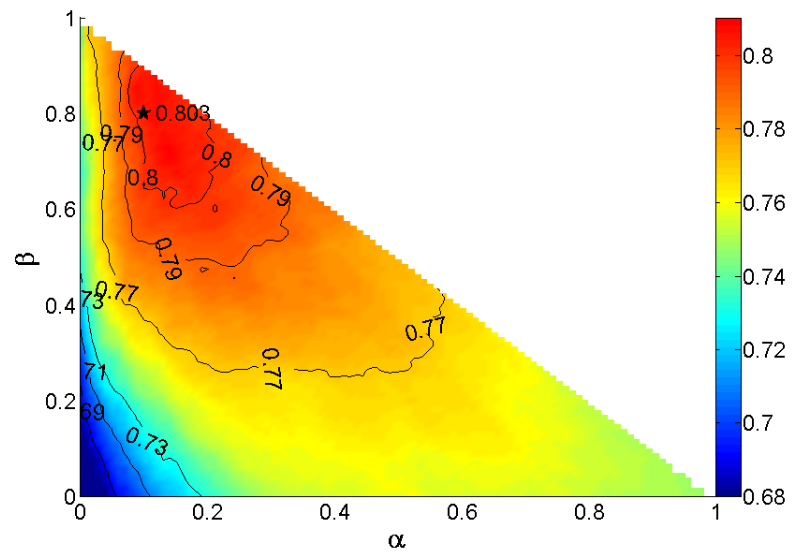
\includegraphics[scale=\graphscaleexpapp]{./exp/AAN-para-recm.eps}}
%\quad\quad
\hspace{\graphmarginexpapp}
\subfigure[{\scriptsize \aminer}]{\label{fig-aminer-ab-recom}
\includegraphics[scale=\graphscaleexpapp]{./exp/AMiner-para-recm.eps}}
%\quad\quad
\hspace{\graphmarginexpapp}
\subfigure[{\scriptsize \magdata}]{\label{fig-mag-ab-recom}
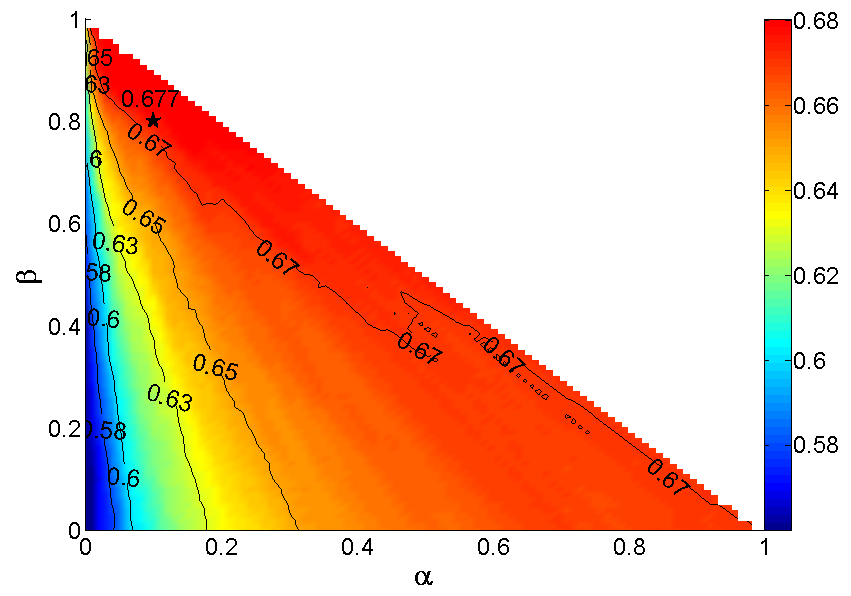
\includegraphics[scale=\graphscaleexpapp]{./exp/MAG-para-recm.eps}}
\\ %%%%%%%%%%%%%%%%%%%%%%%%%%%%%%%%%%%%%%
\vspace{-2ex}
%\hspace{-10ex}
\subfigure[{\scriptsize \aan}]{\label{fig-aan-ab-fcita}
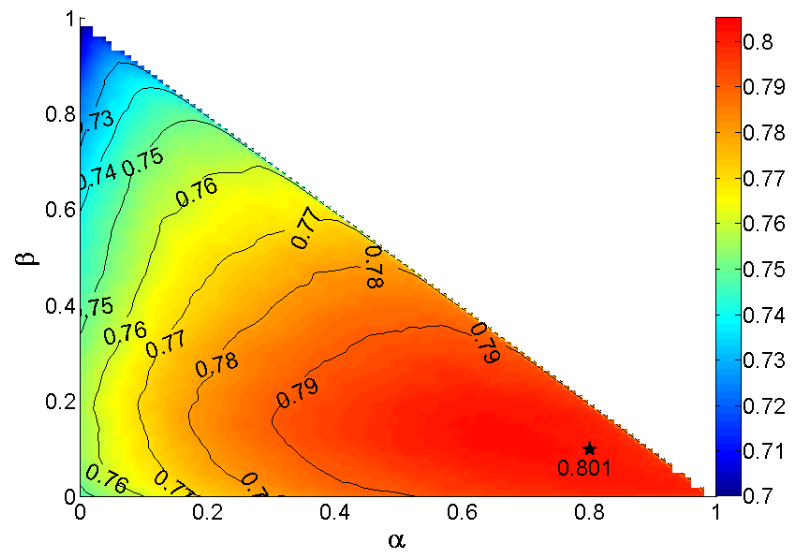
\includegraphics[scale=\graphscaleexpapp]{./exp/AAN-para-fcita.eps}}
%\quad\quad
\hspace{\graphmarginexpapp}
\subfigure[{\scriptsize \aminer}]{\label{fig-aminer-ab-fcita}
\includegraphics[scale=\graphscaleexpapp]{./exp/AMiner-para-fcita.eps}}
%\quad\quad
\hspace{\graphmarginexpapp}
\subfigure[{\scriptsize \magdata}]{\label{fig-mag-ab-fcita}
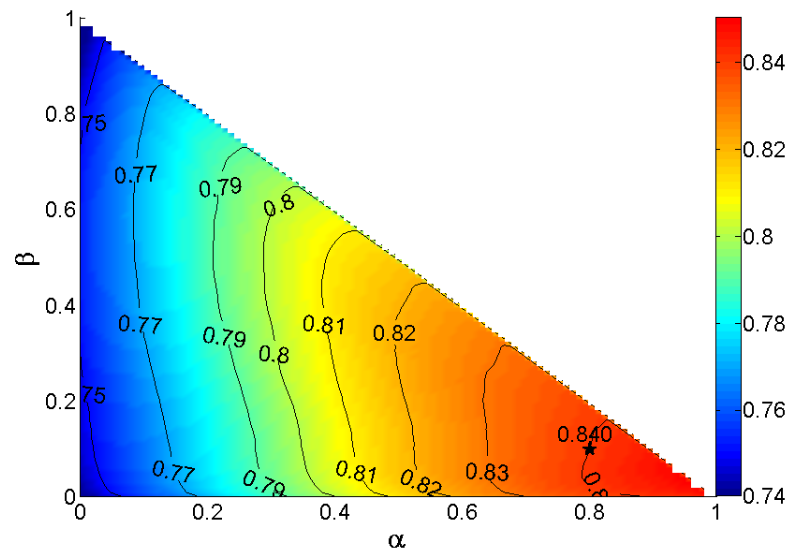
\includegraphics[scale=\graphscaleexpapp]{./exp/MAG-para-fcita.eps}}
\end{center}
\vspace{-3.5ex}
\caption{\small Accuracy tests with \recom ((a)--(c)) and \fcita ((d)--(f)): varying aggregating parameters $\alpha$ and $\beta$}
\label{fig-ab}
\vspace{-3ex}
\end{figure*}
%%%%%%%%%%%%%%%%%%%%%%%%%%%%%%%%%%%%%%

%%%%%%%%%%%%%%%%%%%%%%%%%%%%%%%%%%%%%%%%%%%%%%%%%%
\begin{table}[tb!]
%\vspace{-2ex}
\begin{center}
\begin{small}
\vspace{1ex}
\begin{tabular}{|c|c c c|c c c| c|}
\hline
{\bf Datasets} & {\bf C} & {\bf V} & {\bf A} & {\bf CV} & {\bf CA} & {\bf VA} & {\bf CVA} \\
\hline \hline
% \recom
\aan & 0.746 & 0.616 & 0.647 & 0.806 & 0.760 & 0.746 & {\bf \ 0.810\ } \\
\aminer & 0.783 & 0.576 & 0.664 & 0.805 & 0.798 & 0.735 & {\bf 0.815} \\
\magdata & 0.669 & 0.534 & 0.552 & 0.693 & 0.670 & 0.640 & {\bf 0.694} \\ \hline
% \ficta
\aan & 0.708 & 0.566 & 0.744 & 0.778 & 0.796 & 0.755 & {\bf 0.804} \\
\aminer & 0.690 & 0.733 & 0.761 & 0.854 & 0.839 & 0.794 & {\bf 0.857} \\
\magdata & 0.761 & 0.657 & 0.737 & 0.835 & 0.842 & 0.753 & {\bf 0.849} \\
\hline
\end{tabular}
\end{small}
\end{center}
\caption{\small Accuracy tests on using different components with \recom (rows 2--4) and \fcita (rows 5--7), in which letters C, V and A stand for citation, venue and author components, respectively.}
\label{tab-inc}
\vspace{-6ex}
\end{table}
%%%%%%%%%%%%%%%%%%%



\vspace{-1ex}
\section*{APPENDIX A: Detailed results of Exp-4.3}
\label{sec-exp-app}

%\subsection*{1. Detailed results of Exp-4.3} %$\alpha$ and $\beta$ (detailed)

%We present detailed results of {\em Exp-4.3}, which are omitted earlier due to the space constraints, \ie the impacts of aggregating parameters $\alpha$ and $\beta$ on effectiveness.

\eat{
\etitle{Exp-4.1}. To evaluate the impacts of the time decaying factor $\sigma$, we varied $\sigma$ from -1.6 to -0.4, while fixed $Y_s$ to default values, $b=+\infty$ and $dif=1$. The efficiency results are reported in Fig.~\ref{fig-time-sigma}.
Note that the running time of algorithm \batensemble is different on \recom and \fcita because of the different splitting year $Y_s$.

When varying $\sigma$, the running time of \batensemble is almost stable on both \aminer and \magdata using \fcita and \recom. Indeed, the running time using (\fcita, \recom) only varies (1.4\%, 0.5\%) on \aminer, and (2.1\%, 2.2\%) on \magdata, on average, respectively.
}

\etitle{Exp-4.3}.
To evaluate the impacts of aggregating parameters $\alpha$ and $\beta$, we varied $\alpha$ and $\beta$ at the granularity of 0.01.
The detailed results are reported in Fig.~\ref{fig-ab}, where the parameters selected earlier and their corresponding \PairAcc are marked with $*$.

When varying $\alpha$ and $\beta$, the \PairAcc of \ensemblerank changes gently, as shown in Fig.~\ref{fig-ab}.
The optimal \PairAcc is obtained within a single region, rather than a complex collection of optimal regions.
%
Moreover, the \PairAcc keeps at a high level within a certain ($\alpha$, $\beta$) combination space around the optimal region, as shown in Fig.~\ref{fig-ab}.
%For instance, consider a square of length 0.3, which covers 8.5\% of the parameter combination space. The fraction of parameters such that the \PairAcc is no worse than 1\% of the corresponding \PairAcc with marker $*$ is (73\%, 94\%) on \aan, (96\%, 87\%) on \aminer and (83\%, 95\%) on \magdata, using (\recom, \fcita), respectively.
%
Further, the optimal parameters on the same sets of ground-truth are very similar for (\aan, \aminer and \magdata), indicating that the setting of $\alpha$ and $\beta$ can be easily transferred across different datasets.
To conclude, \ensemblerank is very robust to parameters $\alpha$ and $\beta$, and it is quite flexible for choosing proper values of parameters $\alpha$ and $\beta$.

Moreover, varying $\alpha$ and $\beta$ also enables to verify the effectiveness of importance assembling from different components, whose results are reported in Table~4.
The ranking based on all components consistently performs the best, which, using \recom and \fcita, improves the \PairAcc over using components (C, V, A, CV, CA, VA) by (6.33\%, 19.4\%, 16.3\%, 0.33\%, 4.97\%, 6.33\%) and (9.58\%, 23.8\%, 5.98\%, 2.56\%, 0.74\%, 4.82\%) on \aan, (3.21\%, 23.9\%, 15.1\%, 0.93\%, 1.66\%, 7.97\%) and (16.8\%, 12.5\%, 9.60\%, 0.34\%, 1.87\%, 6.37\%) on \aminer, and ( 2.43\%, 16.0\%, 14.2\%, 0.05\%, 2.38\%, 5.38\%) and (8.89\%, 19.3\%, 11.2\%, 1.43\%, 0.77\%, 9.65\%) on \magdata, respectively.
%Here the letters C, V and A stand for citation component, venue components and author component, respectively.



\section*{APPENDIX B: Detailed Proofs}
\label{sec-proof}

\subsection*{1. Proof of Lemma \ref{prop-nonitercomputing}}

The TWPageRank vector $PR$ returned by \twprdag equals to the convergent TWPageRank vector $PR^*$.

\begin{proof}
We have $PR^* = d M^T\cdot PR^* + \frac{1-d}{n} e$, as $PR^*$ is the convergent TWPageRank vector. Hence, we also have
\begin{small}
\begin{equation}
PR^*(v)=d \sum_{(u,v)\in E^c} M_{u,v} PR^*(u) + \frac{1-d}{n}.
\end{equation}
\end{small}

\vspace{-1ex}
%\noindent

Consider a topological order $v_1/\dots/v_n$ on citation graph $G^c$. We then prove $PR(v_k)=PR^*(v_k)$ ($k\in[1,n]$) by induction.

\noindent(1) When $k=1$, it is obvious that $PR(v_k)=PR^*(v_k)=\frac{1-d}{n}$. %since $PR^*(v_1)=PR(v_1)=\frac{1-d}{n}$;

\noindent(2) Assume that it holds for $1\leq k \leq q$, we then show $PR^*(v_k)=PR(v_k)$ when $k=q+1$ as follows.
\begin{small}
\begin{equation*}
\begin{split}
PR^*(v_{q+1}) & = d \sum_u M_{u,v_{q+1}} PR^*(u) + \frac{1-d}{n} \\
 & = d \sum_u M_{u,v_{q+1}} PR(u) + \frac{1-d}{n}  = PR(v_{q+1}).
\end{split}
\end{equation*}
\end{small}

\vspace{-1ex}
\noindent Here $\{u|(u,v_{q+1})\in E^c\}\subseteq \{v_1,\dots,v_q\}$.
%By these, we have the conclusion.
\end{proof}







\subsection*{2. Proof of Proposition \ref{prop-prscc}}
The TWPageRank vector $PR$ returned by~\twprscc converges such that $||PR-PR^*||_1 < \epsilon$, where $PR^*$ is the convergent TWPageRank vector.

\begin{proof}
%By lemma~\ref{prop-converg}, we know that TWPageRank converges on venue graphs.
We first prove that the sum of changes after another iteration from $PR$ is smaller than $\epsilon$, \ie $||PR^+-PR||_1 < \epsilon$ where $PR^+=d M^T\cdot PR + \frac{1-d}{n} e$, and then prove that $||PR^*-PR||_1$ is smaller than the sum of changes.

Consider $scc_1$, $\dots$, $scc_m$ of the venue graph $G^v$ such that $v_1'/\dots$ $/v_m'$ is indeed a valid topological order of the converted $G'$ of $G^v$, where $m$ is the number of SCCs in $G^v$ and $v_k'$ ($k\in [1,m]$) is the corresponding nodes of $scc_k$ in $G'$.

Let $PR_k$ and $PR_k^-$ be the current and the previous TWPageRank vectors of nodes in $scc_k$ produced
by \twprscc, and $PR_k^+$ be the TWPageRank vector of nodes in $scc_k$ extracted from $PR^+$.
Further let $\Delta_k^-=PR_k-PR_k^-$ and we have:
$\sum_{k=1}^m ||\Delta_k^-||_1 < \epsilon$.

Consider $M_{ij}$ ($i,j\in[1,m]$), the transition submatrix from $scc_i$ to $scc_j$. We have $M_{ij}=\bf{0}$ when $i>j$, since there exists no edges from nodes in later $scc_i$ back to nodes in earlier $scc_j$. And, hence, $PR_k$ and $PR_k^+$ are updated as:
\vspace{-1ex}

\begin{small}
\begin{equation*}
\begin{split}
PR_k=&\frac{1-d}{n} e_k+ d \sum_{j=1}^{k-1} M_{jk}^T PR_j + d M_{kk}^T PR_k^-,\\
PR_k^+=&\frac{1-d}{n}  e_k+ d \sum_{j=1}^{k-1} M_{jk}^T PR_j + d M_{kk}^T PR_k,
\end{split}
\end{equation*}
\end{small}

\vspace{-1ex}
\noindent
respectively, where $e_k=[1]_{|scc_k|\times 1}$.
%, and, obviously, $\Delta_k^+=PR_k^+-PR_k=d M_{kk}^T \Delta_k^-$.

Hence, the sum of changes between $PR^+$ and $PR$ is:

\vspace{-1ex}
\begin{small}
\begin{equation*}
\begin{split}
||PR^+-PR||_1=&\sum_{k=1}^m ||PR_k^+-PR_k||_1=\sum_{k=1}^m ||d M_{kk}^T \Delta_k^-||_1 \\
\le & d\sum_{k=1}^m ||\Delta_k^-||_1 < \epsilon.
\end{split}
\end{equation*}
\end{small}

\vspace{-1ex}
\noindent
based on the fact that the row sums of $M_{kk}$ are always $\le 1$; %less than or equal to 1.

Moreover, $||PR^+-PR||_1 = ||PR^+ - PR^* + PR^* -PR||_1 = ||d M^T (PR-PR^*)||_1 + ||PR-PR^*||_1$, which gives $||PR-PR^*||_1<\epsilon$ and proves the conclusion.
\end{proof}


\subsection*{3. Proof of Proposition \ref{lemma-subgraphA}}
For nodes $v$ within $G^c_A$, $PR^+(v)= PR(v) {n}/{n^+}$.

\begin{proof}
Assume a topological order $v_1/\dots/v_{n_A}$ of graph $G^c_A$ with $n_A=|V^c_A|$.
We prove $PR^+(v_k)={n}/{n^+} PR(v_k)$ ($k\in [1,n_A]$) by induction.
%
Note that given $v\in V^c_A$, $\{(u,v)|(u,v)\in E^{c,+}\}=\{(u,v)|(u,v)\in E^c_A\}$, and, hence, $\Delta M_{u,v} =0$ for $(u,v)\in E^{c,+}$.

\noindent(1) When $k=1$, $PR^+(v_k)={n}/{n^+} PR(v_k)$ obviously holds since $\{(u,v_1)|(u,v_1)\in E^{c,+}\}=\emptyset$;

\noindent(2) Assume that it holds for $1\le k\le q$. We then show $PR^+(v_k)={n}/{n^+} PR(v_k)$ for $k=q+1$, since both ${(n^+-n)}/{n^+} PR(u) + \Delta PR(u)=0$ and $\Delta M_{u,v_{q+1}}=0$ when $(u,v_{q+1})\in E^{c,+}$.
Here $\{u|(u,v_{q+1})\in E^{c,+}\}\subseteq \{v_1,\dots,v_q\}$.
\end{proof}


\subsection*{4. A Stronger Convergence Result}

\eat{
\begin{proof}
%By lemma~\ref{prop-converg}, we know that TWPageRank converges on venue graphs.
It suffices to prove that the sum of changes of TWPageRank vector after another iteration is less than $\epsilon$, \ie $||PR^+-PR||_1 < \epsilon$ where $PR^+=d M^T PR + \frac{1-d}{n} e$.

Consider $scc_1$, $\dots$, $scc_m$ of $G$ such that their corresponding nodes $v_1'$, $\dots$, $v_m'$ are in the topological ordering of the converted DAG of $G$, where $m$ is the number of SCCs in $G$.
Let $PR_k$ and $PR_k^-$ (where $k\in\{1,\dots, m\}$) be the current and the previous TWPageRank vectors of nodes in $scc_k$ produced by \twprscc. Further let $\Delta_k^-=PR_k-PR_k^-$ and we have:
$\sum_{k=1}^m ||\Delta_k^-||_1 < \epsilon$.
Similarly, let $PR_k^+$ be the TWPageRank vectors of nodes in $scc_k$ extracted from $PR^+$.

Let $M_{ij}$ be the transition submatrix denoting the transition from $scc_i$ to $scc_j$, where $i,j\in \{1,\dots, m\}$. We have $M_{ij}=\bf{0}$ when $i>j$, since these exists no edges from later $scc_i$ back to early $scc_j$. And, hence, $PR_k$ and $PR_k^+$ are updated as:
\vspace{-1ex}

\begin{small}
\begin{equation*}
\begin{split}
PR_k=&\frac{1-d}{n}+ d \sum_{j=1}^{k-1} M_{jk}^T PR_j + d M_{kk}^T PR_k^-,\\
PR_k^+=&\frac{1-d}{n}+ d \sum_{j=1}^{k-1} M_{jk}^T PR_j + d M_{kk}^T PR_k,
\end{split}
\end{equation*}
\end{small}

\vspace{-1ex}
\noindent
respectively. Hence, $\Delta_k^+=PR_k^+-PR_k=d\cdot M_{kk}^T \Delta_k^-$.

The sum of changes between $PR^+$ and $PR$ is:

\vspace{-1ex}
\begin{small}
\begin{equation*}
\begin{split}
||PR^+-PR||_1=&\sum_{k=1}^m ||\Delta_k^+||_1=\sum_{k=1}^m ||d M_{kk}^T \Delta_k^-||_1 \\
\le & d\sum_{k=1}^m ||\Delta_k^-||_1 < \epsilon.
\end{split}
\end{equation*}
\end{small}

\vspace{-1ex}
\noindent
based on the fact that the row sums of $M_{kk}$ are always less than or equal to 1.
\end{proof}
}  %%%%% eat proof




\begin{figure}[tb!]
\centering
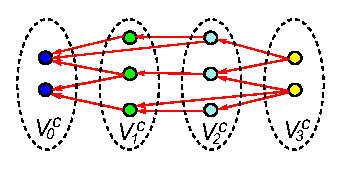
\includegraphics[scale=.8]{fig/DAG_Layers.eps}
\vspace{-2ex}
\caption{An example of a four-layer citation graph}
\label{fig-daglayers}
\vspace{-2ex}
\end{figure}


Proposotion~\ref{prop-converg} has shown the convergence of TWPageRank. We further present a stronger convergence result giving the number of iterations needed for power method to achieve convergence, which is based on dividing citation graphs into ordered layers.

Since the citation graph $G^c(V^c,E^c)$ can be treated as a directed acyclic graph, $V^c$ can be organized into ordered layers such that all edges are from later layers to earlier layers. To do this, let $l_v$ be the length of the longest path starting from node $v$,
%Such values for all nodes in $G$ can be computed in linear time~\cite{SedgewickW11}, by finding a topological ordering of $G$ and updating the length $l_v$ of each node $v$ in the topological ordering.
and $L$ be the length of the longest path starting from any node in $G^c$, \ie $L = \max_{v\in V^c} l_v$. Based on $l_v$,  $V^c$ is then divided into $L+1$ disjoint layers $V^c_0,V^c_1,\dots,V^c_{L}$ such that $V^c_0\bigcup V^c_1 \bigcup \dots \bigcup V^c_{L}=V^c$ and node $v\in V^c_{k}$ iff $l_v=k$. %($k\in[0,L]$).

\begin{example}
\label{eg-layer-dag}
Fig.~\ref{fig-daglayers} illustrates a four-layer citation graph, where $L$ equals to the length of the longest path, \ie 3, and the nodes are divided into 4 layers $[V^c_0, \ldots, V^c_3]$, such that $V^c_{k}$ ($k\in[0,3]$) contains all nodes starting from whom the length of the longest path is exactly $k$, and all edges are from  $V^c_i$ to $V^c_j$ where $i>j$.
\end{example}

\eat{
For the convenience of notation, we first rewrite the PageRank update rule in Eq.~(\ref{eq-twpr}) into matrix form:

\begin{small}
\begin{equation}
PR^{(t)}=d M^T \cdot PR^{(t-1)} + \frac{1-d}{n} e.
\end{equation}
\end{small}

\vspace{-1ex}
\noindent
Here $PR^{(t-1)}$ and $PR^{(t)}$ %, consisting of PageRank scores of all nodes,
are PageRank vectors after $t-1$ and $t$ iterations, respectively, $M$ is the transition matrix such that $M_{u,v}=w(u,v)/W(u)$ and $e$ is a $n$-dimentional vector $[1]_{n\times1}$.
}


\begin{prop} \label{prop-strong-conv}
TWPageRank converges to a unique vector on an $(L+1)$-layer citation graph after $L+1$ iterations, regardless of the initial vector.
\end{prop}

\begin{proof}
Given the initial TWPageRank vector $PR^{(0)}$, the PageRank vector after $t$ iterations is:
\vspace{-1ex}

\begin{small}
\begin{equation}
\label{eq-noniterpr}
%\begin{split}
PR^{(t)} =  d^t (M^T)^t PR^{(0)} + \frac{1-d}{n} \sum_{k=1}^{t-1}(d M^T)^k e +\frac{1-d}{n} e,
%\end{split}
\end{equation}
\end{small}

\vspace{-1ex}
\noindent
which is derived by iteratively computing $PR^{(1)}$ up to $PR^{(t)}$.

Without loss of generality, we consider $G^c$ whose nodes are properly arranged  such that nodes in $V^c_0$ come first, followed by ones in $V^c_1$ till $V^c_{L}$. In this case the transition matrix $M$ of $G^c$ is a strictly lower triangular matrix since all edges are from  $V^c_i$ to $V^c_j$ where $i>j$. Moreover, $M^{L+1}=\textbf{0}$.

When $t\ge L+1$, the first term in the right hand of Eq.~(\ref{eq-noniterpr}) becomes $\textbf{0}$, and $PR^{(t)}$ equals to
$\frac{1-d}{n} \sum_{k=1}^{L}(d M^T)^k e +\frac{1-d}{n} e$,
which is the unique convergent TWPageRank vector of $G^c$, regardless of the initial vector $PR^{(0)}$.
\end{proof}

%
\begin{figure*}[tb!]
%\vspace{-2ex}
\begin{center}
%\hspace{10ex}
\subfigure[{\scriptsize \aan)}]{\label{fig-aan-lambda}
\includegraphics[scale=0.38]{./exp/AAN_lambda.eps}}
%\quad\quad
\hspace{\graphmargin}
\subfigure[{\scriptsize \aminer}]{\label{fig-aminer-lambda}
\includegraphics[scale=0.38]{./exp/AMiner_lambda.eps}}
%\quad\quad
\hspace{\graphmargin}
\subfigure[{\scriptsize \magdata)}]{\label{fig-mag-lambda}
\includegraphics[scale=0.38]{./exp/MAG_lambda.eps}}
\end{center}
\vspace{-5ex}
\caption{\small Accuracy tests: varying importance weighting parameter $\lambda$}
\label{fig-lambda}
\vspace{-3ex}
\end{figure*}



\vspace{-1ex}
\section*{APPENDIX C: Further Experiments}
\label{sec-exp-app2}


\subsection*{1. Exp-5: Impacts of the importance weighting scheme on effectiveness}

Recall that the prestige and popularity are equally weighted to produce the importance by default in Eq.~(\ref{eq-imp}). In the fifth of tests, we further evaluated the impacts of the importance weighting scheme on effectiveness. To do this, we introduced the importance weighting parameter $\lambda$ such that $\lambda \in [0,1]$ and rewrote Eq.~(\ref{eq-imp}) as $Imp_c(v) = Prs_c(v)^\lambda \cdot Pop_c(v)^{1-\lambda}$, where $\lambda$ and $1-\lambda$ control the contributions of prestige and popularity to produce importance, respectively.
We varied $\lambda$ from 0 to 1, while fixed $Y_s$ to default values, $b=+\infty$, $dif=1$ and $\sigma=-1.0$. The results of the \PairAcc on both benchmarks are reported in Fig.~\ref{fig-lambda}. Note that parameter $\lambda$ has no impacts on efficiency.

When varying $\lambda$, the \PairAcc of \ensemblerank first increases and then decreases on all datasets using both benchmarks. This result indicated that our importance model combining both prestige and popularity is better than using either of prestige and popularity alone. The selection of $\lambda$ is influenced by benchmarks, such that the best $\lambda$ falls into $[xx,xx]$ and $[yy,yy]$ on \fcita and \recom, respectively. Moreover, equally weighting, \ie $\lambda=0.5$, is a good default setting when no query information is available in advance.
Indeed, the best obtained \PairAcc using (\fcita, \recom) is only (0.10\%, 0.38\%), (0.04\%, 2.59\%) and (0.06\%, 0.91\%)  higher than the \PairAcc of equally weighting on \aan, \aminer and \magdata, respectively. 


